\documentclass[tikz,border=10pt]{standalone}
% Shared look for every TikZ diagram. Load with \input{../../tools/tikz-style.tex}
\usepackage[T1]{fontenc}
\usepackage{lmodern}
\renewcommand{\sfdefault}{lmr}  % diagrams use the same serif as the text
\usetikzlibrary{arrows.meta, positioning, shapes.geometric, calc, fit, backgrounds}
\definecolor{cblue}{HTML}{4C78A8}
\definecolor{corange}{HTML}{F58518}
\definecolor{cgreen}{HTML}{54A24B}
\definecolor{cred}{HTML}{E45756}
\definecolor{cpurple}{HTML}{B279A2}
\definecolor{cgrey}{HTML}{6B6B6B}
\tikzset{
  every picture/.style={font=\sffamily, line width=1.2pt},
  box/.style={draw=#1, fill=#1!12, rounded corners=4pt, align=center, inner sep=7pt, minimum height=1.1cm},
  box/.default=cgrey,
  arrow/.style={-{Stealth[length=3mm]}, draw=cgrey, line width=1.4pt},
  title/.style={font=\sffamily\bfseries\Large},
  note/.style={font=\sffamily\small, text=cgrey, align=center},
}
\AtBeginDocument{\hyphenpenalty=10000 \exhyphenpenalty=10000}

\begin{document}
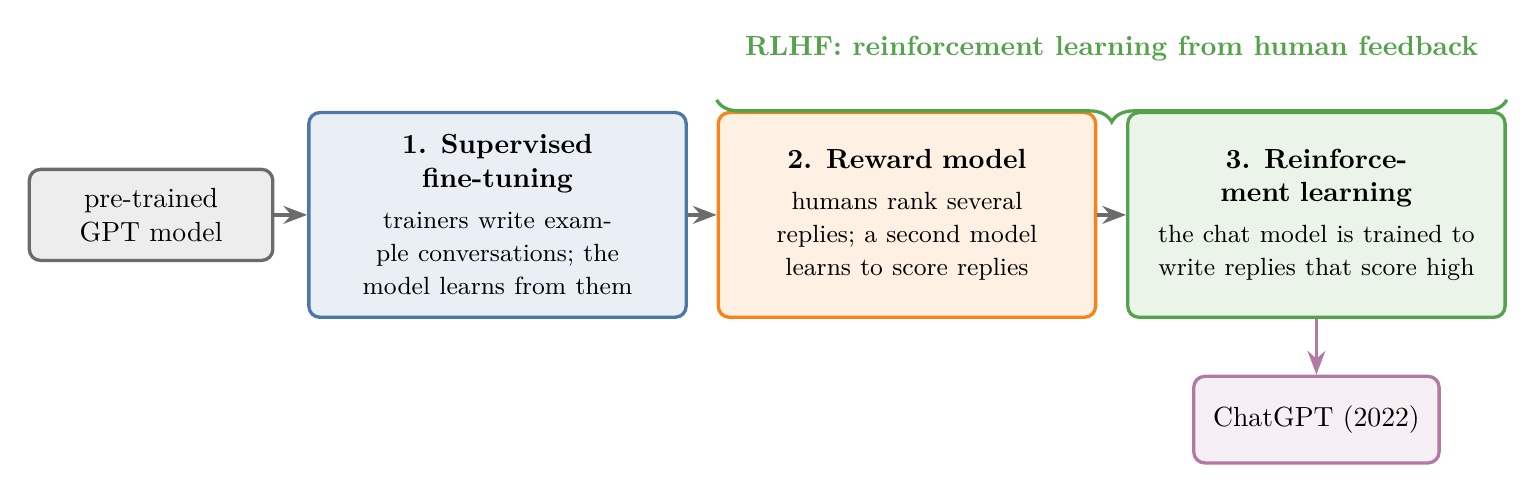
\begin{tikzpicture}[st/.style={box=#1, text width=4.3cm, minimum height=2.6cm, font=\sffamily}]
  \node[box=cgrey, text width=2.6cm] (g) at (0,0) {pre-trained\\GPT model};
  \node[st=cblue] (s1) at (4.4,0) {\textbf{1. Supervised fine-tuning}\\[3pt]\small trainers write example conversations; the model learns from them};
  \node[st=corange] (s2) at (9.6,0) {\textbf{2. Reward model}\\[3pt]\small humans rank several replies; a second model learns to score replies};
  \node[st=cgreen] (s3) at (14.8,0) {\textbf{3. Reinforcement learning}\\[3pt]\small the chat model is trained to write replies that score high};
  \draw[arrow] (g) -- (s1); \draw[arrow] (s1) -- (s2); \draw[arrow] (s2) -- (s3);
  \draw[decorate, decoration={brace, amplitude=8pt}, cgreen] ([yshift=4pt]s3.north east) -- node[above=10pt, font=\sffamily\bfseries, text=cgreen] {RLHF: reinforcement learning from human feedback} ([yshift=4pt]s2.north west);
  \node[box=cpurple] (c) at (14.8,-2.6) {ChatGPT (2022)};
  \draw[arrow, draw=cpurple] (s3.south) -- (c.north);
\end{tikzpicture}
\end{document}
